\section{Evaluating Effects of Barium Sulfate\label{sec:methodology:effectsOfBaSO4}}

\subsection{Imaging Study\label{sec:methodology:effectsOfBaSO4:imagingStudy}}

A predominant goal of the barium sulfate extrusions and printing was to evaluate its effects on radiopacity. To measure these effects, an imaging study was conducted. This study was conducted in collaboration with the Stephanie Spielman Comprehensive Breast Center (OSUCCC).

\subsubsection{Sample Preparation\label{sec:methodology:effectsOfBaSO4:imagingStudy:samplePrep}}

Samples were prepared based on similar conducted literature~\cite{RefWorks:RefID:77-hamedani2018threedimensional}. A $1cm$ wide and $1cm$ tall cylinder was designed in SolidWorks, and numerous samples were printed for each barium sulfate concentration group. Based on supply of extruded filament, four samples were printed for each concentration group.

To eliminate air gaps, samples were printed with 100\% infill.

The various 3D printed samples for imaging are shown below in Figure~\ref{fig:methodology:effectsOfBaSO4:imagingStudySamples}

\begin{figure}[h!]
        \centering
        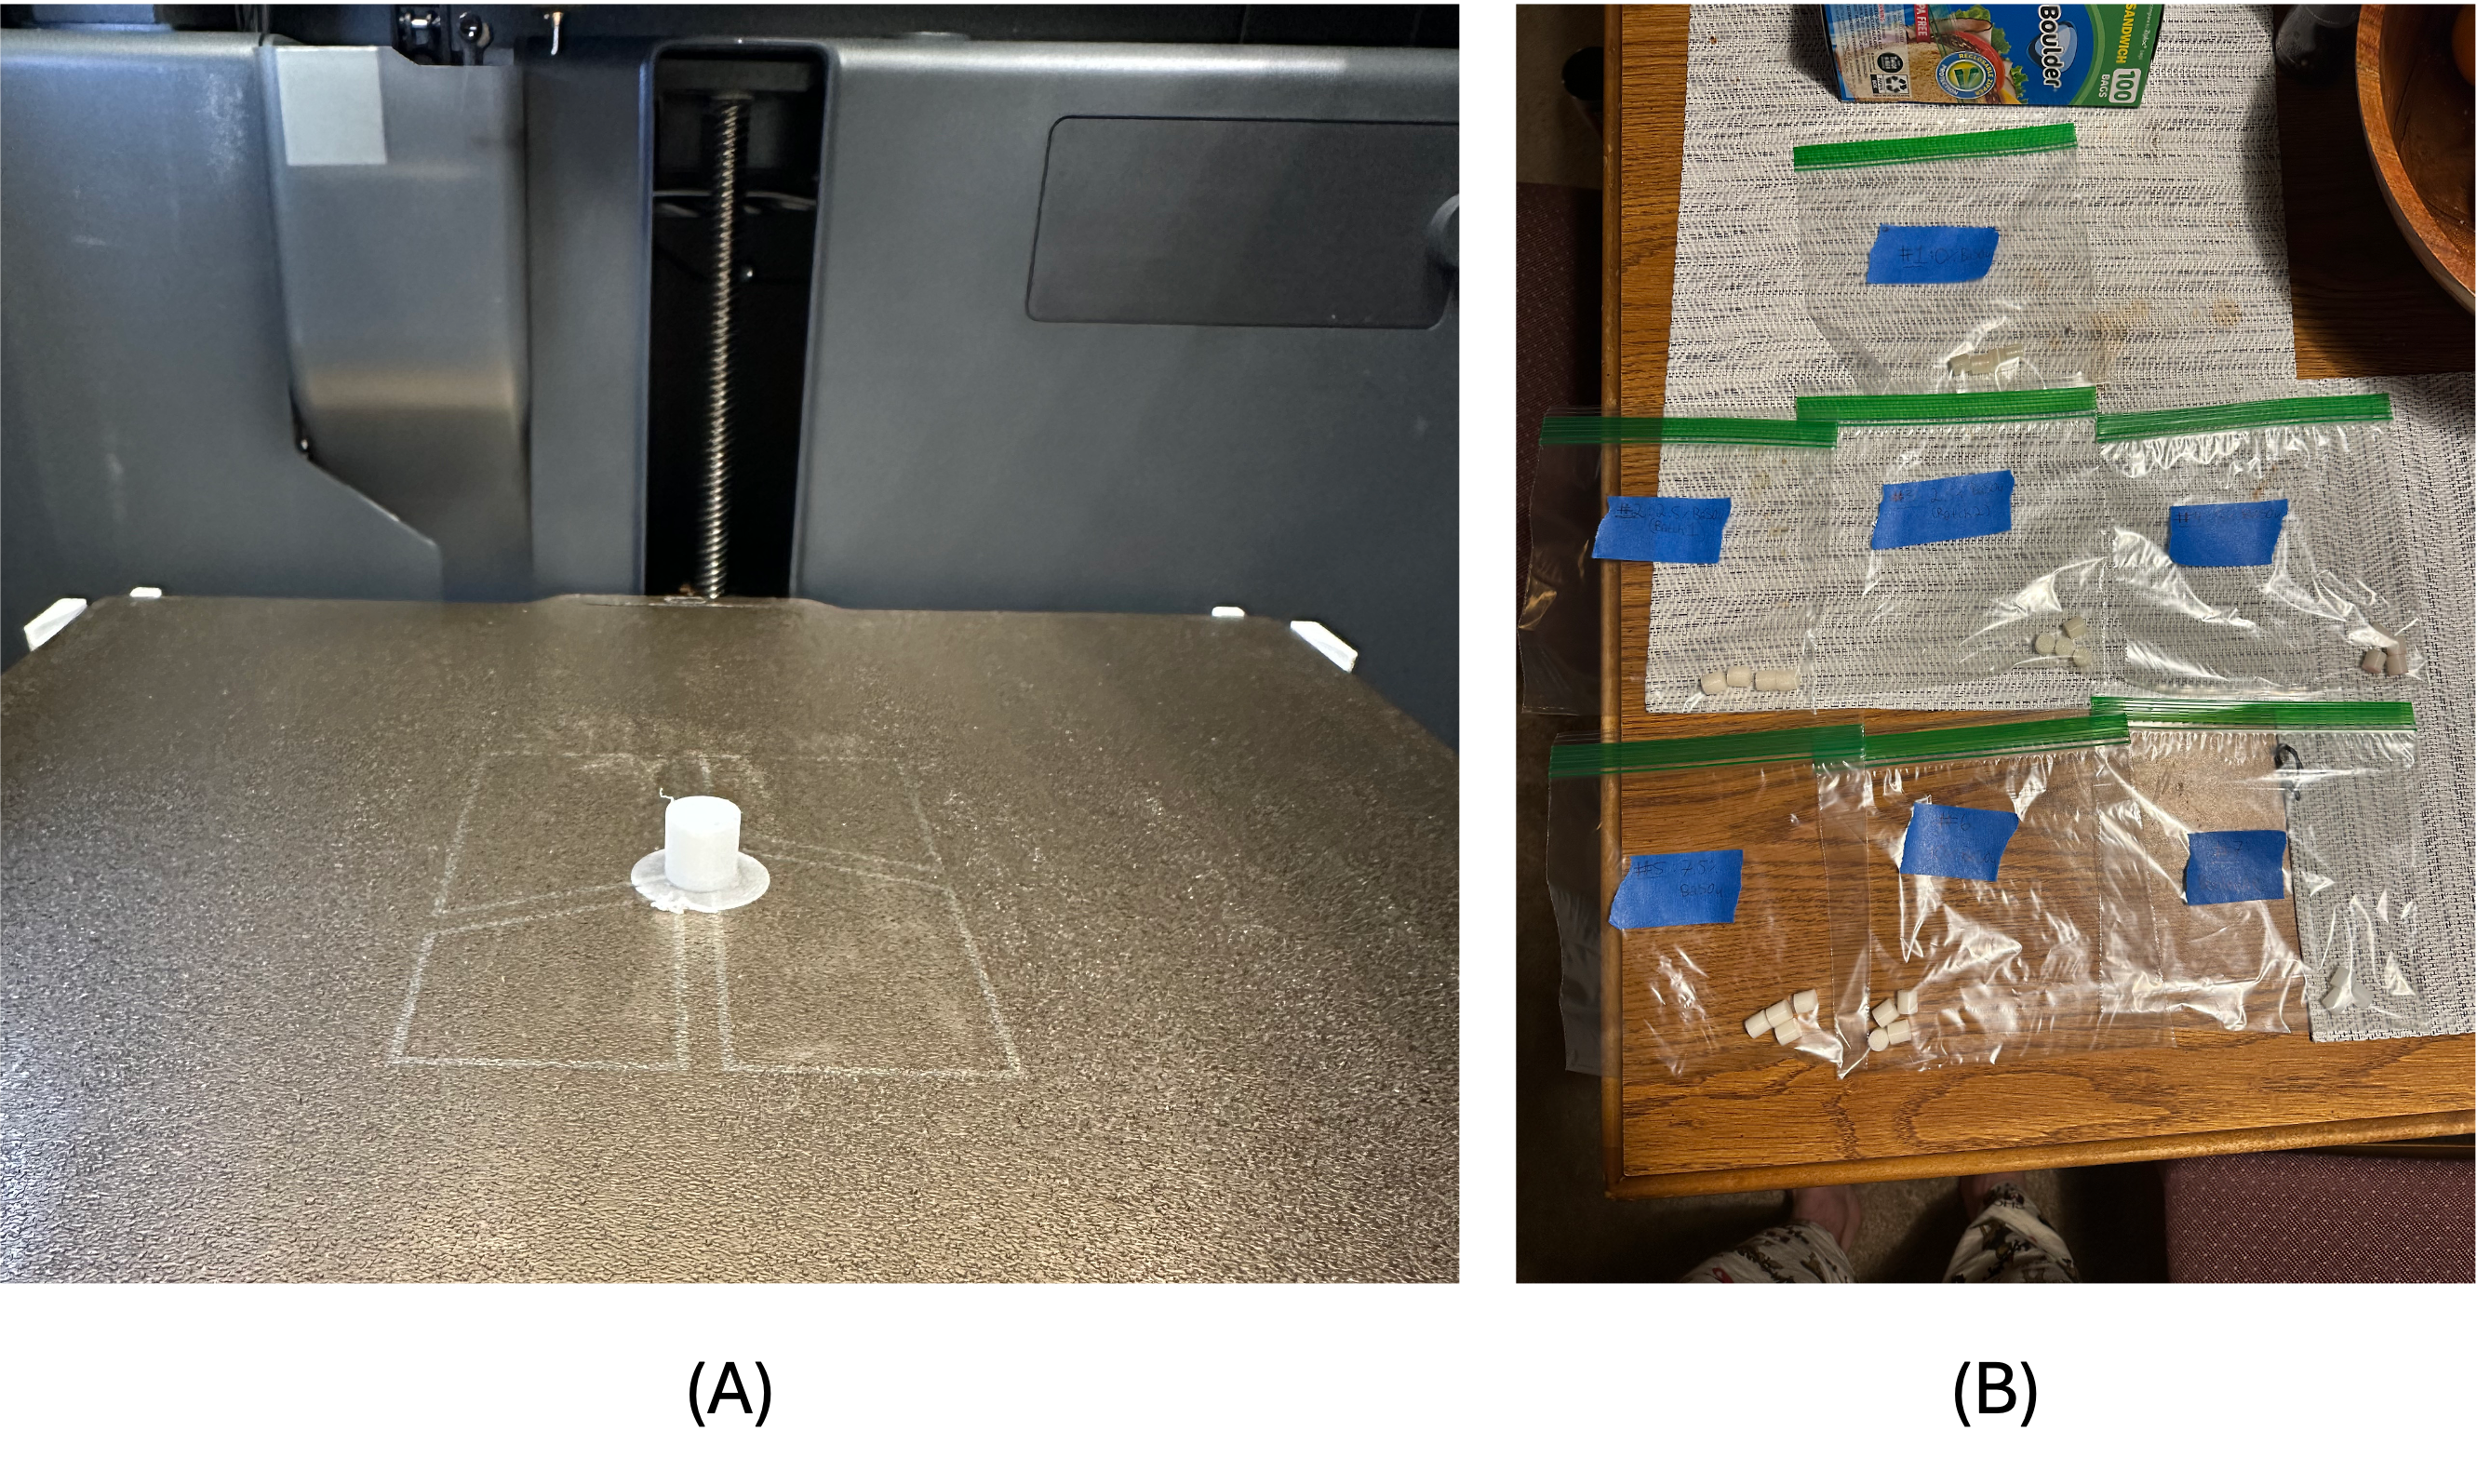
\includegraphics[width=\linewidth]{../figs/methodology/imagingStudy/imaging_study_samples.png}
        \caption{Imaging study samples. Individual printed sample (A) and all final bagged samples (B).}
        \label{fig:methodology:effectsOfBaSO4:imagingStudySamples}
\end{figure}

\subsubsection{Bonlecule Filament\label{sec:methodology:effectsOfBaSO4:imagingStudy:bonlecule}}

In addition to the custom-made PLA/BaSO\textsubscript{4} filaments, a commercially made radiopaque filament, Bonlecule, was also tested. A sample of this filament was sent from NOVUS~\cite{RefWorks:RefID:78-bonlecule}.

To 3D print Bonlecule, printing parameters from the manufacturer were used based initially on PLA Marble presets. Table~\ref{tab:methodology:bonleculeParameters} summarizes the final printing parameters used for this filament. Additionally, following manufacturer suggestions, glue was applied to the build plate to improve build plate adhesion.

Due to limited filament initially supplied, three samples of Bonlecule filament rather than four were printed for this imaging study.

\begin{table}[h!]
        \centering
        \caption{Printing parameters for Bonlecule filament.}
        \label{tab:methodology:bonleculeParameters}
        \begin{adjustbox}{max width=\textwidth}
                \begin{tabular}{l l l l l c c c c c c l c c c c c}
                        \hline
                        \textbf{Base Material}                        &
                        \textbf{Vendor/Extruder}                      &
                        \textbf{Initial Preset}                       &
                        \textbf{BaSO$_4$ \%}                          &
                        \textbf{Nozzle Size (mm)}                     &
                        \textbf{Initial Layer}                        &
                        \textbf{Initial layer infill}                 &
                        \textbf{Outer wall}                           &
                        \textbf{Inner wall}                           &
                        \textbf{Sparse infill}                        &
                        \textbf{Internal solid infill}                &
                        \textbf{Recommended Nozzle Temperature Range} &
                        \textbf{Textured PEI Plate Initial Layer}     &
                        \textbf{Textured PEI Plate Other Layers}      &
                        \textbf{Nozzle Initial Layer}                 &
                        \textbf{Nozzle Other Layers}                  &
                        \textbf{Max Volumetric Speed (mm$^3$/s)}                                                                                                                                      \\
                        \hline

                        Unknown                                       & Bonlecule & PLA Marble & Unknown & 0.6 Cold Hardened\% & 35 & 55 & 120 & 150 & 120 & 150 & 220--240 & 85 & 85 & 230 & 230 & 8 \\

                        \hline
                \end{tabular}
        \end{adjustbox}
\end{table}

Samples were given to OSUCCC where Dr. Eric Cochran helped image all samples.

Results and discussion of this imaging study can be found in~\fullref{sec:results:effectsOfBaSO4:imagingStudy} and~\fullref{sec:discussion:effectsOfBaSO4:imagingStudy} respectively.

\subsection{Tensile Testing\label{sec:methodology:effectsOfBaSO4:tensileTesting}}

\subsection{Flexural Testing\label{sec:methodology:effectsOfBaSO4:flexuralTesting}}
